\usetikzlibrary{arrows.meta,calc}
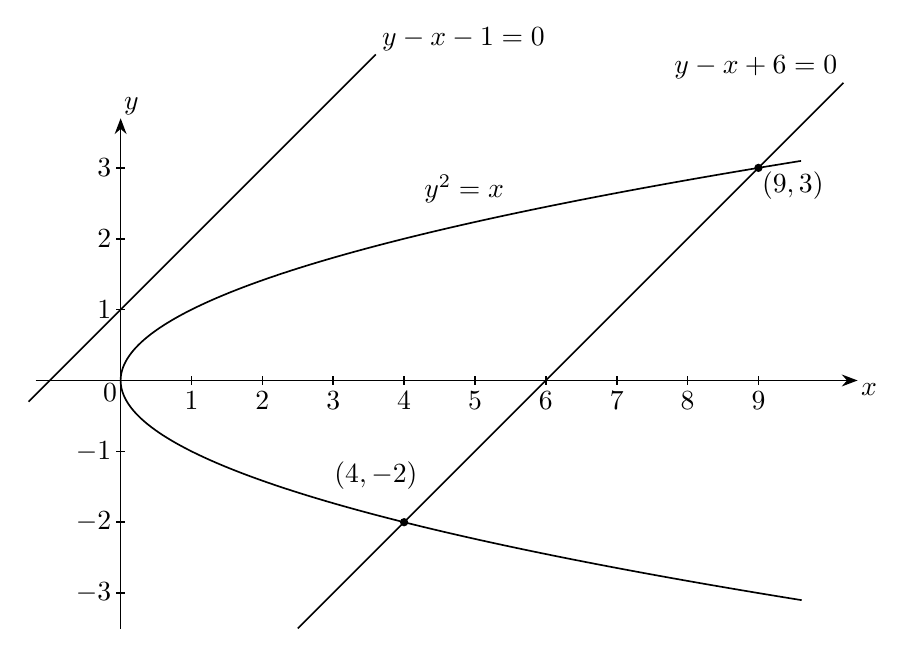
\begin{tikzpicture}[x=0.9cm,y=0.9cm,line width=.6pt,font=\normalsize,>=Stealth]
\coordinate (O) at (0,0);
\coordinate (Qone) at (9,3);
\coordinate (Qtwo) at (4,-2);
\coordinate (Pgiven) at (8,2);
\coordinate (XaxisStart) at (-1.2,0);
\coordinate (XaxisEnd) at (10.4,0);
\coordinate (YaxisStart) at (0,-3.5);
\coordinate (YaxisEnd) at (0,3.7);
\coordinate (LoneStart) at (-1.3,-0.3);
\coordinate (LoneEnd) at (3.6,4.6);
\coordinate (LtwoStart) at (2.5,-3.5);
\coordinate (LtwoEnd) at (10.2,4.2);
% axes
\draw[->] (XaxisStart)--(XaxisEnd) node[below right,inner sep=0pt,xshift=1pt,yshift=-1pt] {$x$};
\draw[->] (YaxisStart)--(YaxisEnd) node[above right,inner sep=0pt,xshift=1pt,yshift=1pt] {$y$};
\foreach \k in {1,...,9} {\draw (\k,0.06)--(\k,-0.06); \node[below,inner sep=0pt] at (\k,-0.15) {$\k$};}
\foreach \m in {-3,-2,-1,1,2,3} {\draw (0.06,\m)--(-0.06,\m); \node[left,inner sep=0pt] at (-0.12,\m) {$\m$};}
\node[below left,inner sep=0pt,xshift=-1pt,yshift=-1pt] at (O) {$0$};
% curve and lines
\draw[domain=-3.1:3.1,samples=161] plot ({(\x)^2},\x);
\draw (LoneStart)--(LoneEnd);
\draw (LtwoStart)--(LtwoEnd);
% intersection points
\fill (Qone) circle (1.5pt);
\fill (Qtwo) circle (1.5pt);
% labels
\node[below right,inner sep=0pt,xshift=1pt,yshift=-1pt] at (Qone) {$(9,3)$};
\node[above left,inner sep=0pt] at (4.2,-1.55) {$(4,-2)$};
\node[above left,inner sep=0pt,xshift=-2pt,yshift=1pt] at (5.5,2.45) {$y^2=x$};
\node[above right,inner sep=0pt,xshift=2pt,yshift=1pt] at (3.6,4.6) {$y-x-1=0$};
\node[above left,inner sep=0pt,xshift=-2pt,yshift=1pt] at (10.2,4.2) {$y-x+6=0$};
\end{tikzpicture}
